\ifdefined\ishandout
    \documentclass[handout]{beamer}
\else
    \documentclass{beamer}
    \setbeamercovered{transparent}
\fi

\includeonly{git}

\usepackage{selthcsslides}
\usecolortheme{lucolors}

% \usepackage[swedish]{babel}
% Swedish setup using polyglossia for better multilingual support
\usepackage{polyglossia}
\setmainlanguage{swedish}

\usepackage{url}
\usepackage{datetime2}

\usepackage{fontspec}  			  % Allows loading system fonts
\setmainfont{Latin Modern Roman}  % Set the main (serif) font
\setsansfont{Latin Modern Roman}  % Force sans-serif font to use the same font


\author[]{Mattias Nordahl}
\institute{\url{mattias.nordahl@cs.lth.se}}
\date{} 

%***************************************************************
\begin{document} 

\title{Datorer och datoranvändning\\Introduktion} 

\frame[plain]{
\maketitle

\vspace{-2\baselineskip}
}

\date{\the\year/\the\numexpr\year-1999} 

% Include actual slides


\begin{frame}
    \frametitle{Vad är versionshantering?}

    \begin{itemize}
        \ii{Har du någonsin... }
        \begin{itemize}
            \ii{Mejlat filer fram och tillbaka med ändringar?}
            \ii{Förlorat en viktig fil eller version av ditt arbete?}
            \ii{Skrivit över en fil av misstag?}
            \ii{Behövt hålla koll på olika versioner av samma dokument?}
        \end{itemize}
        \ii{Versionshantering hjälper dig att hantera dessa problem!}
    \end{itemize}
\end{frame}


\begin{frame}
    \frametitle{Versionshanteringssystem}

    \begin{block}{Vad är ett versionshanteringssystem?}
        \halfblankline
        \ti{Ett verktyg för att göra versionshantering enklare, genom att spåra och hantera ändringar i projektfiler över tid.}
        \halfblankline
    \end{block}

    \begin{itemize}
        \ii{Spårbarhet -- vem som gjort vad och när. T.ex.:}
        \begin{itemize}
            \ii{\enquote{Vad har ändrats sedan förra veckan?}}
            \ii{\enquote{Vem la till den här raden?}}
        \end{itemize}
        \ii{Möjlighet att återgå till äldre versioner av filer vid behov.}
        \ii{Möjliggör parallellt arbete och konflikthantering.}
    \end{itemize}

\end{frame}

\begin{frame}
    \frametitle{Typer av versionshanteringssystem (1/2)}

    \begin{block}{Centraliserade system}
        \begin{itemize}
            \ii{En central server lagrar alla filer och versioner. (\emph{repository})}
            \ii{Användare hämtar \textbf{en} version, ändrar, och sparar tillbaka den.}
            \ii{Kommandon: \emph{checkout} (hämta filer), \emph{commit} (spara till servern).}
            \ii{Exempel: Subversion (SVN), Perforce}
        \end{itemize}
    \end{block}

\end{frame}

\begin{frame}
    \frametitle{Centraliserad versionshantering}

    \begin{center}
        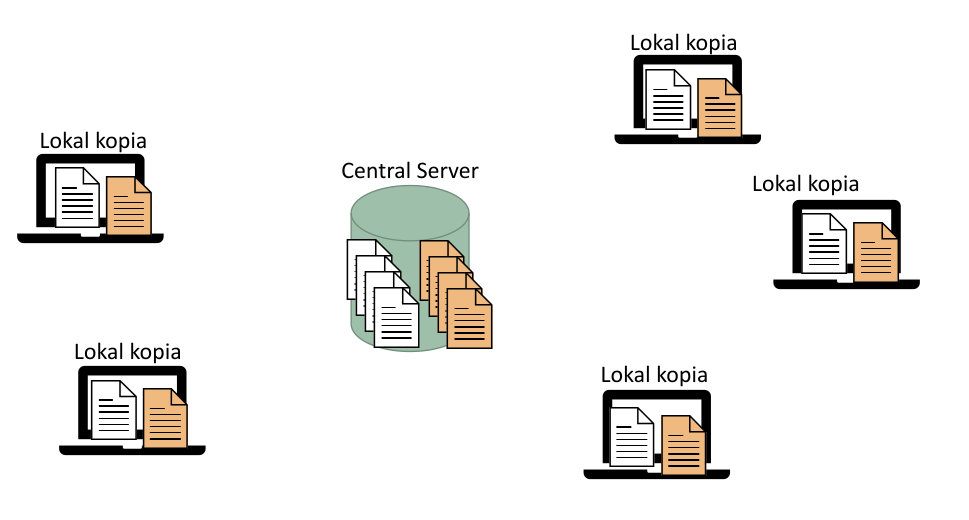
\includegraphics[width=0.80\textwidth]{figs/fig1_central_model.png}
    \end{center}
\end{frame}

\begin{frame}
    \frametitle{Typer av versionshanteringssystem (2/2)}

    \begin{block}{Distribuerade system}
        \begin{itemize}
            \ii{Ingen central server -- varje användare är en \enquote{nod} i systemet.}
            \ii{Varje användare har en lokal kopia av hela projektets historik.}
            \ii{Kommandon: \emph{clone} (kopiera hela repository), \emph{checkout} och \emph{commit} (men annorlunda), och \emph{push/pull} (synkronisera ändringar).}
            \ii{Exempel: Git, Mercurial}
        \end{itemize}
    \end{block}

\end{frame}

\begin{frame}
    \frametitle{Distrubuerad versionshantering}

    \begin{center}
        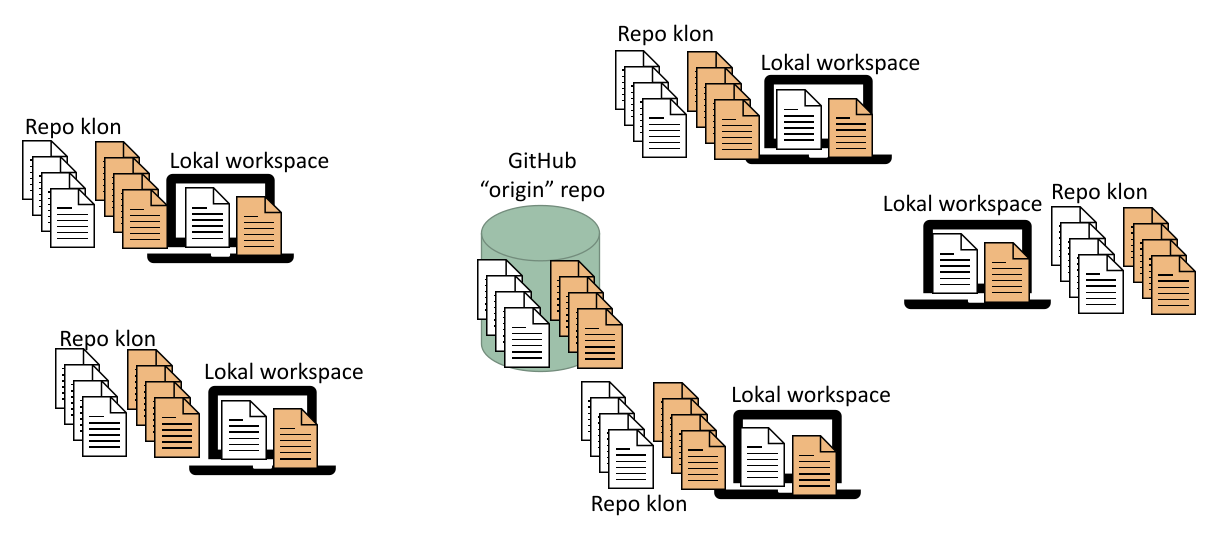
\includegraphics[width=\textwidth]{figs/fig2_git_model.png}
    \end{center}
\end{frame}

\begin{frame}
    \frametitle{Introduktion till Git}

    \begin{itemize}
        \ii{\emph{Git} är ett distribuerat versionshanteringssystem.}
        \ii{Utvecklat av Linus Torvalds 2005. \url{https://github.com/git/git}}
        \ii{Designat för snabb hantering av projekt med många bidragsgivare.}
        \ii{Används av de flesta moderna mjukvaruprojekt och open source-projekt.}
        \ii{Ger full kontroll över historik, branchning, och sammanslagning av ändringar (\emph{merging}).}
    \end{itemize}

    \blankline
    \ti{Testa: \code{git rev-list --max-parents=0 HEAD}}

\end{frame}

\begin{frame}
    \frametitle{Git vs. GitHub: Vad är skillnaden?}

    \begin{block}{Git}
        \begin{itemize}
            \ii{Ett \emph{verktyg} för versionshantering som körs lokalt på din dator.}
        \end{itemize}
    \end{block}

    \begin{block}{GitHub}
        \begin{itemize}
            \ii{En \emph{tjänst} för att hosta Git-repositories online.}
            \ii{Underlättar samarbete med andra utvecklare genom att erbjuda funktioner som pull requests, issues och projektöversikt.}
            \ii{Använder Git internt för att hantera repositories, precis som lokala installationer av Git.}
        \end{itemize}
    \end{block}

\end{frame}

\begin{frame}
    \frametitle{Grundläggande Git-kommandon}

    \begin{description}
        \di{git init}{Initierar ett nytt Git-repository lokalt.}
        \di{git clone}{Kopierar ett existerande repository (t.ex. från GitHub) till din dator.}
        \di{git add}{Lägger till ändringar i staging-området inför nästa commit.}
        \di{git commit}{Sparar ändringar lokalt med en beskrivande kommentar.}
        \di{git push}{Laddar upp dina lokala ändringar till ett fjärrrepository (t.ex. GitHub).}
        \di{git pull}{Hämtar och integrerar ändringar från ett fjärrrepository.}
    \end{description}

\end{frame}


\begin{frame}
    \frametitle{Git-modellen}

    \begin{itemize}
        \ii{\emph{Workspace}: En vanlig mapp på datorn där du jobbar med filer.}
        \ii{\emph{Staging Area}: En "kopia" av workspace där du förbereder ändringar inför nästa sparning.}
        \ii{\emph{Repository}: Ett arkiv som lagrar alla tidigare versioner av projektet.}
    \end{itemize}

    \begin{center}
        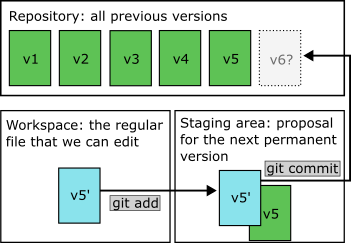
\includegraphics[height=.5\textheight]{figs/model-add-commit.png}
    \end{center}

\end{frame}

\begin{frame}
    \frametitle{Vad är en Commit?}

    \begin{minipage}{0.7\textwidth}
        \begin{itemize}
            \ii{En \emph{commit} är en "ögonblicksbild" (\emph{snapshot}) av projektet vid ett specifikt tillfälle.}
            \ii{Innehåller alla ändringar som gjorts sedan den senaste commiten.}
            \ii{Varje commit refererar till sin(a) föregångare och skapar en historik.}
            \ii{Bildar en graf av versioner som visar projektets utveckling över tid.}
        \end{itemize}
    \end{minipage}
    \hspace{.05\textwidth}
    \begin{minipage}{0.20\textwidth}
        \begin{center}
            \begin{tikzpicture}
                % Draw the vertical line
                \draw[thick] (0, 0) -- (0, 3);

                % Draw the commit nodes
                \foreach \y in {0, 1, 2, 3} {
                        \filldraw (0, \y) circle (3pt);
                    }

                % Label the commits
                \node[right, xshift=5pt] at (0, 3) {Commit 1};
                \node[right, xshift=5pt] at (0, 2) {Commit 2};
                \node[right, xshift=5pt] at (0, 1) {Commit 3};
                \node[right, xshift=5pt] at (0, 0) {Commit 4};
            \end{tikzpicture}

        \end{center}
    \end{minipage}

\end{frame}

\begin{frame}
    \frametitle{Grenar (\emph{Branches})}

    \begin{minipage}{0.7\textwidth}

        \ti{Man kan skapa parallella utvecklingsgrenar, som sedan kan slås samman (\emph{merge}) med huvudgrenen igen.}

        \begin{itemize}
            \ii{Varför vill man göra det?}
            \ii{Vilka problem kan uppstå?}
        \end{itemize}
    \end{minipage}
    \hspace{.05\textwidth}
    \begin{minipage}{0.20\textwidth}
        \begin{tikzpicture}
            % Rita huvudgrenen (main)
            \draw[thick] (0, 0) -- (0, 5);
            \foreach \y in {0, 1, 3, 4, 5} {
                    \filldraw (0, \y) circle (3pt);
                }
            \node[above, yshift=2pt] at (0, 5) {\emph{main}};

            % Rita parallellgrenen (branch)
            \draw[thick] (0, 4) -- (1, 3) -- (1, 2) -- (0, 1);
            \foreach \y in {2, 3} {
                    \filldraw (1, \y) circle (3pt);
                }
            \node[above, yshift=2pt, xshift=15pt] at (1, 3) {\emph{branch}};
        \end{tikzpicture}
    \end{minipage}

\end{frame}

\begin{frame}
    \frametitle{Varför grenar (\emph{branches})?}

    \begin{itemize}
        \ii{Grenar = parallella vägar; sidospår utan att störa huvudvägen.}
        \ii{Arbeta på olika delar av projektet samtidigt, utan att störa varandra.}
        \ii{Testa nya funktioner, experimentera säkert.}
        \ii{Skapa snabb fix för fel utan att stoppa ny utveckling.}
        \ii{Branches i Git är lätta att skapa och använda!}
    \end{itemize}

\end{frame}

\begin{frame}
    \frametitle{Vilka problem kan uppstå?}

    \begin{itemize}
        \ii{\emph{Merge}: Git kombinerar ändringar från olika grenar automatiskt.}
        \ii{\emph{Merge-konflikt}: Uppstår när Git inte kan avgöra hur vissa ändringar ska kombineras.}
        \ii{Konflikter sker ofta när samma del av en fil ändrats på flera grenar.}
        \ii{Exempel: Flera redigerar samma rad, eller ändrar/byter namn på samma filer.}
        \ii{Konflikter måste lösas manuellt för att slutföra en \emph{merge}.}
    \end{itemize}

\end{frame}

\begin{frame}[fragile]
    \frametitle{Exempel: Merge-konflikt i källkoden}

    \begin{block}{\small Kod före merge}
        \begin{GobbleCode}[0pt]{10}
            def greet(): String = {
                "Hello, world!"
            }
        \end{GobbleCode}
    \end{block}

    \begin{block}{\small Kod efter merge (med konflikt)}
        \begin{GobbleCode}[0pt]{10}
            def greet(): String = {
            <<<<<<< HEAD
                "Hello, world!"
            =======
                "Hi, everyone!"
            >>>>>>> branch
            }
        \end{GobbleCode}
    \end{block}

    \begin{itemize}
        \ii{Konflikten visas med \texttt{<<<<<<<}, \texttt{=======}, och \texttt{>>>>>>>}.}
        \ii{Utvecklaren måste välja vilken version som ska behållas eller kombinera dem manuellt.}
    \end{itemize}

\end{frame}


\begin{frame}[fragile]
    \frametitle{Ett större exempel}

    \begin{GobbleCode}[2pt]{6}
        object Main {
            def main(args: Array[String]): Unit = {
                println("Starting calculation...")
                println("Result: " + calculateSum(5, 10))
            }

            def calculateSum(a: Int, b: Int): Int = {
        <<<<<<< HEAD
                val sum = a + b
                println("Sum calculated: " + sum)
                sum
        =======
                val sum = a + b
                println("Calculating sum for: " + a + " and " + b)
                println("Sum is: " + sum)
                sum * 2 // Doubles the result
        >>>>>>> branch
            }
        }
    \end{GobbleCode}

\end{frame}

\begin{frame}
    \frametitle{Arbeta distribuerat med Git}

    \begin{itemize}
        \ii{\emph{Klona}: Kopiera ett repository från internet till din dator.}
        \ii{\emph{Pull}: Hämta ändringar från ett fjärrrepository.}
        \ii{\emph{Push}: Skicka dina ändringar till ett fjärrrepository.}
        \ii{\emph{Pull request}: Föreslå ändringar till ett repository.}
        \begin{itemize}
            \ii{Mycket vanligt i \emph{open source}-projekt.}
            \ii{Kallas ibland \emph{merge request}.}
        \end{itemize}
    \end{itemize}

\end{frame}

\begin{frame}
    \frametitle{Remote}

    \begin{itemize}
        \ii{Git använder termen \emph{remote}. Lokal \enquote{spegling} av fjärrrepository.}
        \ii{Standardnamn för remote är \texttt{origin}.}
        \ii{Möjligt att ha flera remotes för olika kopior av projektet.}
        \ii{Kolla med \texttt{git remote [-a, -v, -vv]}}
    \end{itemize}

\end{frame}

\begin{frame}
    \frametitle{Påminnelse - Context}

    \begin{center}
        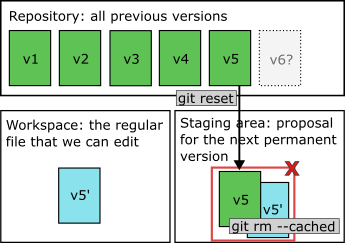
\includegraphics[height=.5\textheight]{figs/model-rm-reset.png}
    \end{center}

\end{frame}

\begin{frame}
    \frametitle{Local vs remote: commit och push}

    \begin{center}
        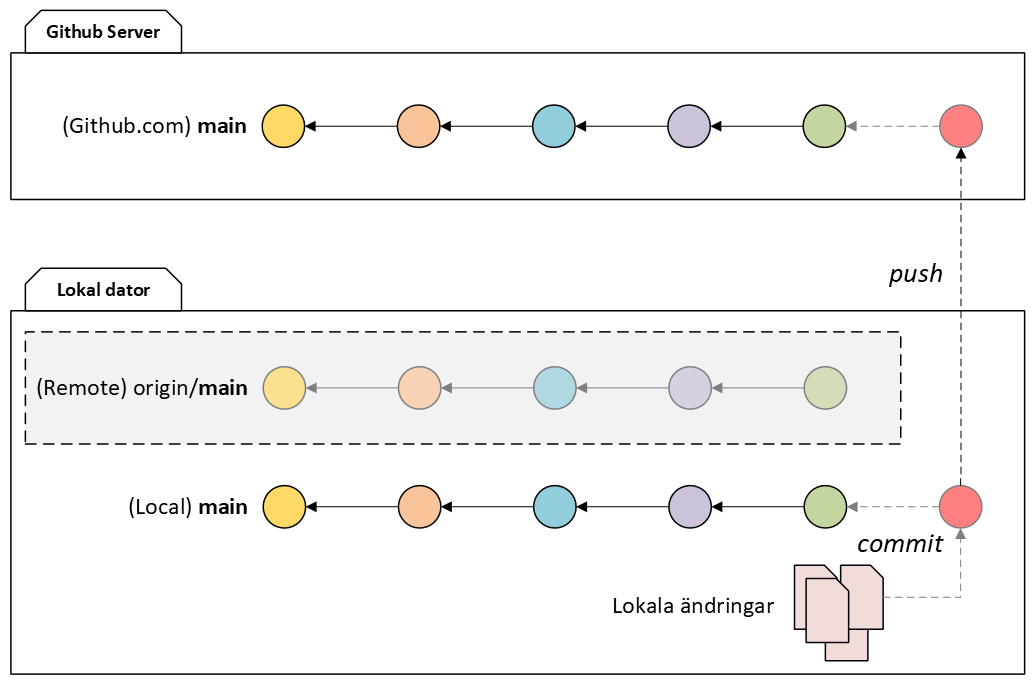
\includegraphics[width=.9\textwidth]{figs/local_remote_commit_push.png}
    \end{center}

\end{frame}

\begin{frame}
    \frametitle{Local vs remote: fetch och merge}

    \begin{center}
        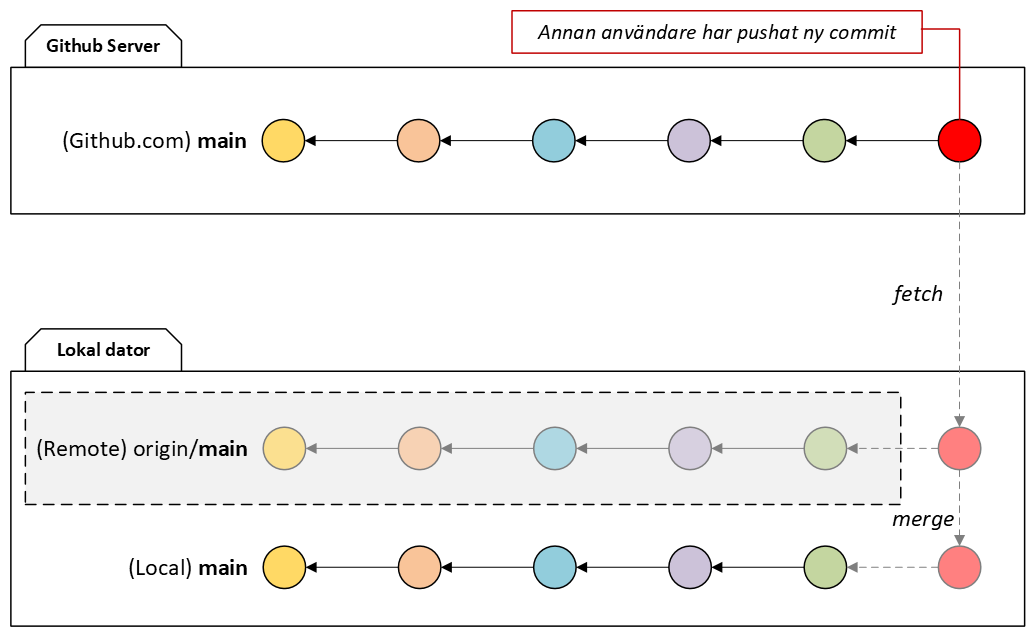
\includegraphics[width=.9\textwidth]{figs/local_remote_fetch_merge.png}
    \end{center}

\end{frame}

\begin{frame}
    \frametitle{Båda samtidigt!? -- push}

    \begin{center}
        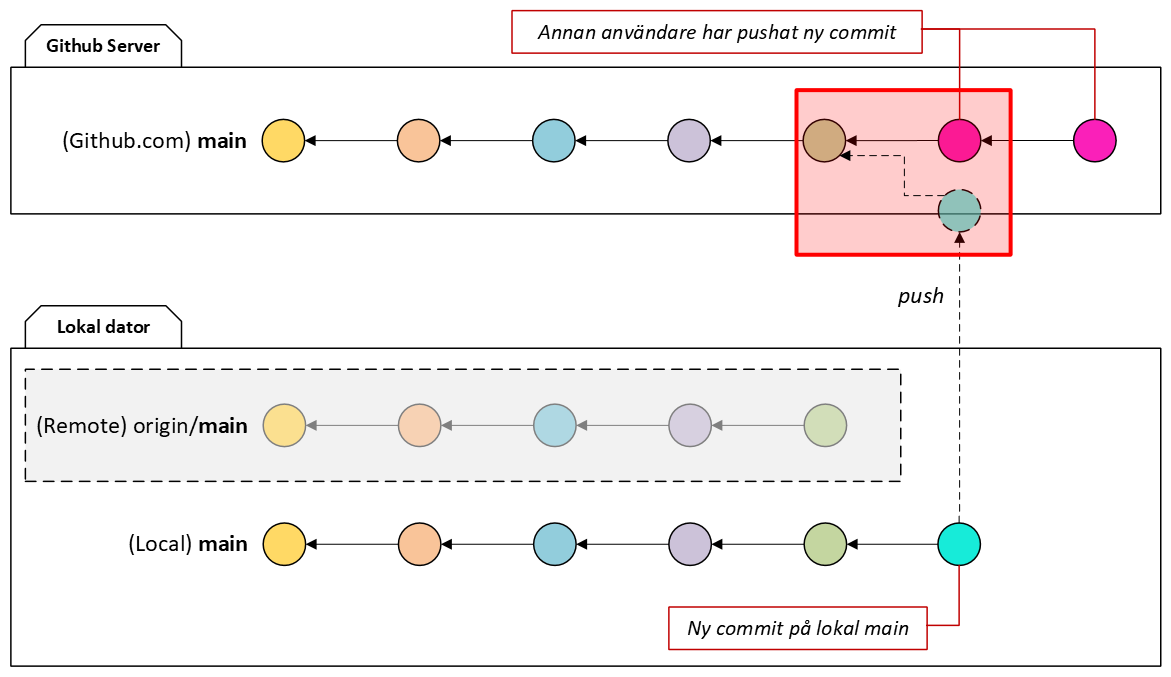
\includegraphics[width=\textwidth]{figs/local_remote_push_conflict.png}
    \end{center}

\end{frame}

\begin{frame}
    \frametitle{Båda samtidigt!? -- fetch}

    \begin{center}
        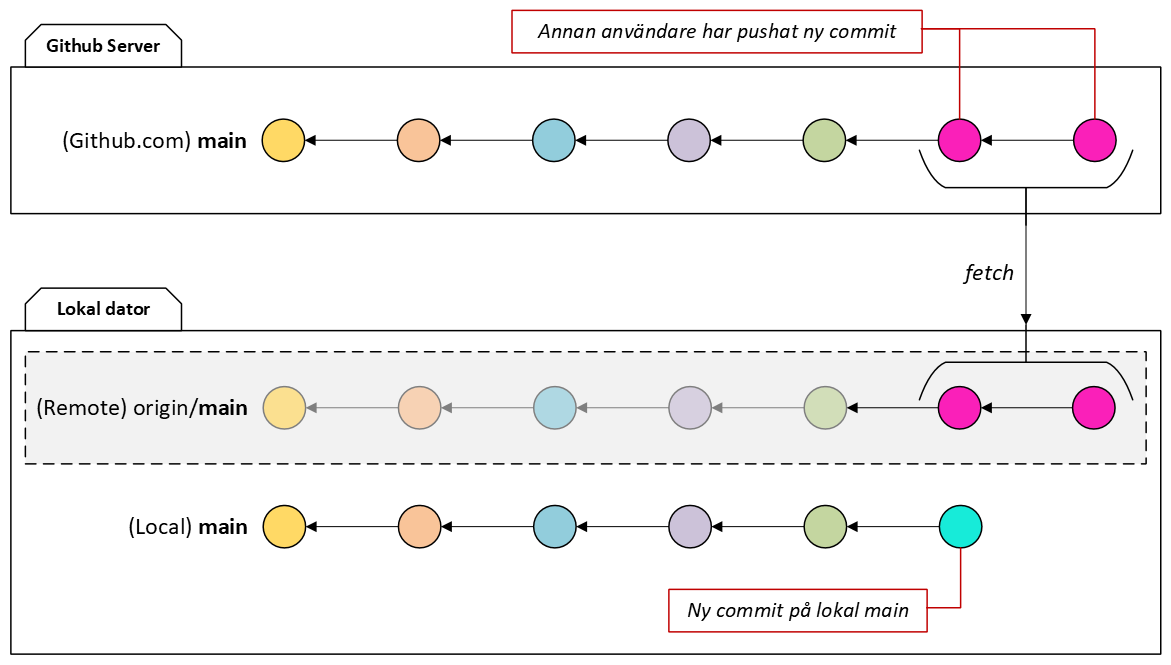
\includegraphics[width=\textwidth]{figs/local_remote_fetch_conflict.png}
    \end{center}

\end{frame}

\begin{frame}
    \frametitle{Båda samtidigt!? -- merge efter fetch}

    \begin{center}
        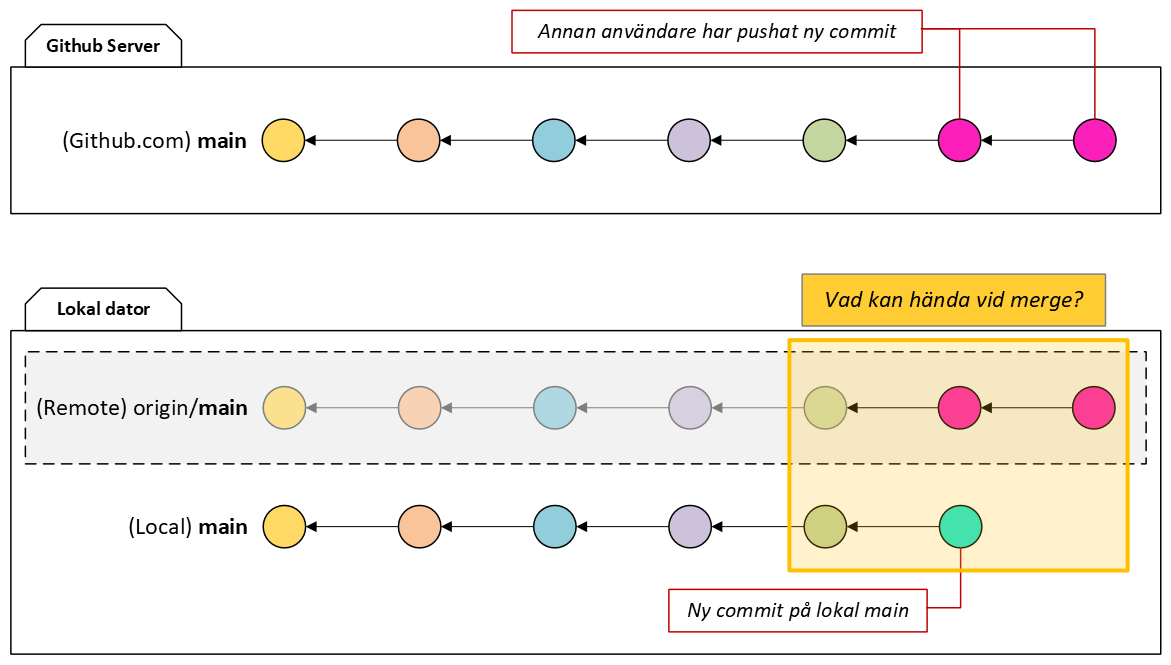
\includegraphics[width=\textwidth]{figs/local_remote_fetch_merge_conflict.png}
    \end{center}

\end{frame}


\begin{frame}
    \frametitle{Merge-situationer}

    \ti{Vad kan hända vid merge?}
    \begin{itemize}
        \ii{fast-forward merge}
        \ii{merge commit}
        \ii{konflikt}
        \ii{rebase}
    \end{itemize}

\end{frame}

\begin{frame}[t]
    \frametitle{Fast-forward merge}
    \vspace{-1.5em}
    \begin{center}
        \begin{tikzpicture}
            % Place the image at 50% scale
            \node (img) at (0, 0) {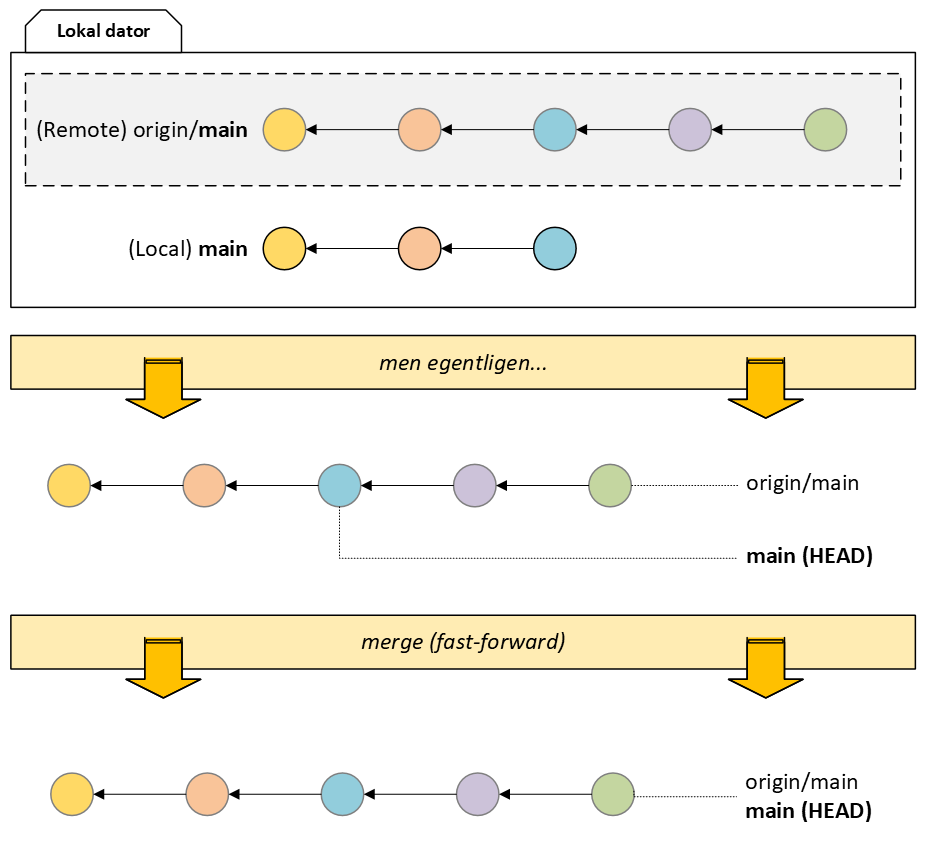
\includegraphics[scale=0.5]{figs/merge_case_ff.png}};

            % Only show partial overlays in the presentation mode
            \mode<beamer>{
                % Overlay 1: Cover the lower 2/3 of the image with a white box
                \only<1>{
                    \fill[white] ([yshift=-0.33\textheight]img.north west) rectangle (img.south east);
                }
                % % Overlay 2: Cover the lower 1/3 of the image with a white box
                \only<2>{
                    \fill[white] ([yshift=-0.6\textheight]img.north west) rectangle (img.south east);
                }
                % Overlay 3: Show the full image (no white box needed)
                \uncover<3>{
                    % No white box, full image visible
                }
            }
        \end{tikzpicture}
    \end{center}
\end{frame}

\begin{frame}[t]
    \frametitle{Vanlig merge -- skapar en \enquote{merge commit}}
    \begin{center}
        \begin{tikzpicture}
            % Place the image at 50% scale
            \node (img) at (0, 0) {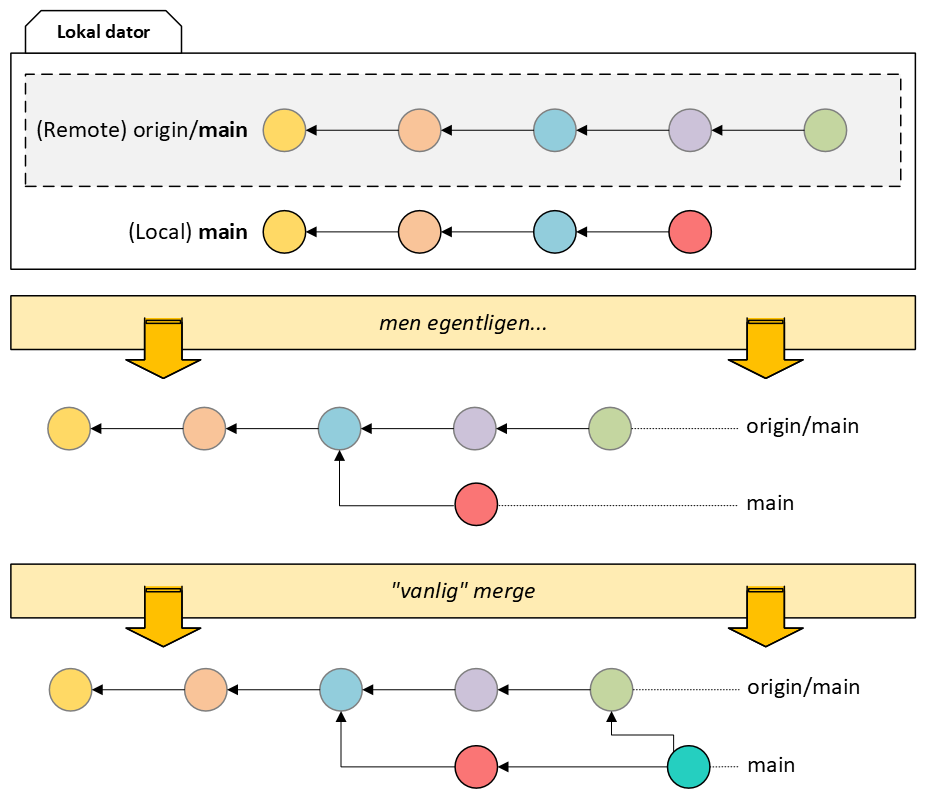
\includegraphics[scale=0.5]{figs/merge_case_commit.png}};

            % Only show partial overlays in the presentation mode
            \mode<beamer>{
                % Overlay 1: Cover the lower 2/3 of the image with a white box
                \only<1>{
                    \fill[white] ([yshift=-0.28\textheight]img.north west) rectangle (img.south east);
                }
                % % Overlay 2: Cover the lower 1/3 of the image with a white box
                \only<2>{
                    \fill[white] ([yshift=-0.55\textheight]img.north west) rectangle (img.south east);
                }
                % Overlay 3: Show the full image (no white box needed)
                \uncover<3>{
                    % No white box, full image visible
                }
            }
        \end{tikzpicture}
    \end{center}
\end{frame}

\begin{frame}
    \frametitle{Mergekonflikt}
    \ti{Vid konflikt, se föregående figur.}
    \begin{itemize}
        \ii{Om ändringarna i de två grenarna inte kan kombineras automatiskt, uppstår en konflikt.}
        \ii{Git markerar konflikter i filerna och pausar merge-processen.}
        \ii{Efter konflikten lösts, finns alltså ny ändringar i worspace\dots}
        \ii{...och du måste göra en ny commit för att slutföra merge.}
    \end{itemize}

\end{frame}

\begin{frame}[t]
    \frametitle{Rebase}
    \vspace{-.5em}
    \begin{center}
        \begin{tikzpicture}
            % Place the image at 50% scale
            \node (img) at (0, 0) {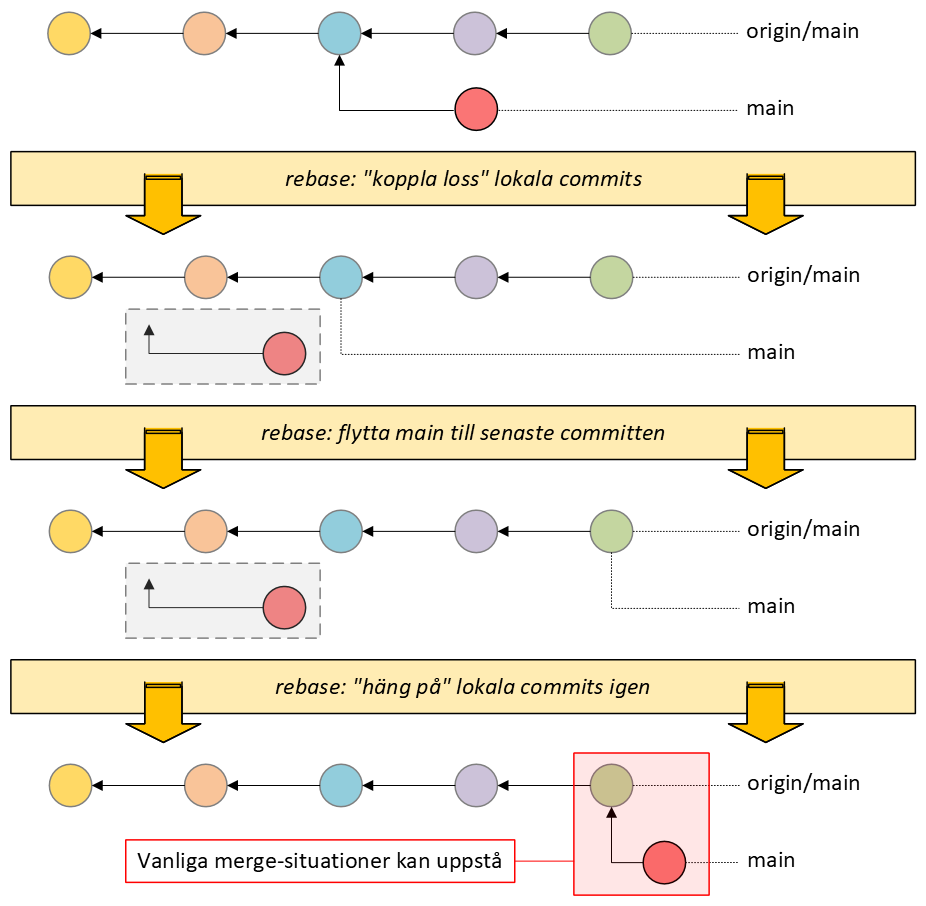
\includegraphics[scale=0.46]{figs/merge_case_rebase.png}};

            % Only show partial overlays in the presentation mode
            \mode<beamer>{
                % Overlay 1: Cover the lower 2/3 of the image with a white box
                \only<1>{
                    \fill[white] ([yshift=-0.14\textheight]img.north west) rectangle (img.south east);
                }
                % % Overlay 2: Cover the lower 1/3 of the image with a white box
                \only<2>{
                    \fill[white] ([yshift=-0.36\textheight]img.north west) rectangle (img.south east);
                }
                % % Overlay 3: Cover the lower 1/3 of the image with a white box
                \only<3>{
                    \fill[white] ([yshift=-0.59\textheight]img.north west) rectangle (img.south east);
                }
                % Overlay 4: Show the full image (no white box needed)
                \uncover<4>{
                    % No white box, full image visible
                }
            }
        \end{tikzpicture}
    \end{center}
\end{frame}



\begin{frame}
    \frametitle{Bra att veta}

    \begin{itemize}
        \ii{\code{HEAD} är en \emph{symbolisk referens} till den branch som är utcheckad i ditt workspace.}
        \ii{\enquote{Detatched HEAD} -- om du checkar ut en specifik commit, snarare än en branch.}
    \end{itemize}
\end{frame}

\begin{frame}
    \frametitle{Veckans laboration}

    \ti{På veckans laboration kommer ni:}
    \begin{itemize}
        \ii{Arbeta er igenom ett enkelt scenario som visar hur ni kan använda Git och Github för ett litet projekt.}
        \ii{Tänkt att kunna genomföras individuellt, men OK och uppmuntras till att samarbeta, speciellt i den sista delen av laborationen.}
    \end{itemize}

    \halfblankline
    \ti{Glöm inte att:}
    \begin{itemize}
        \ii{Installera Git på din egen dator.}
    \end{itemize}

\end{frame}

\begin{frame}
    \frametitle{Vad händer nu?}
    \begin{itemize}
        \ii{Läs avsnittet om Git i Scalakompendiet (Björn Regnell).}
        \ii{Se avsnitt 1.1, 1.2, 1.3, 1.6 samt 1.7 av youtube-serien \enquote{Git and GitHub for Poets}.}
        \ii{Läs kapitel 1, 2 och 3.1--3.2 i Pro Git-boken (Chacon \& Straub).}
        \ii{Länkar till materialet finns på kurshemsidan:

            \halfblankline
            \url{https://lunduniversity.github.io/pgk}}
    \end{itemize}

\end{frame}


\end{document} 
